\chapter{Interface}

A interface de comunicação do seu sistema deve atender os seguintes requisitos da \autoref{tabela-interface}:

\begin{table}[htb]
\IBGEtab{
  \caption{Especificação de Dados}
  \label{tabela-interface}
}{
  \begin{tabular}{ccc}
  \toprule
   Nome & Tipo & Tamanho em bits \\
  \midrule \midrule
   Valid & Entrada & 1 \\
  \midrule 
   DataIn & Entrada & 32 \\
  \midrule 
   Ready & Saída & 1 \\
  \midrule 
   DataOut & Saída & 321 \\
  \bottomrule
\end{tabular}
}{
  \fonte{Produzido pelos autores.}%
  \nota{Ready será levado para 1 quando o IP estiver pronto para entrada ou saída de dados.}
  \nota{Valid só será ativado quando o ready estiver levantado e servirá para a entrada de dados.}
  \nota{DataIn só será gravado quando o Valid e o Ready estiverem ativos.}
  }
\end{table}

Na \autoref{fig-maquina-estados} você pode analisar a maquina de estados do sistema.
\par
\begin{figure}[htb]
    \caption{\label{fig-maquina-estados}Maquina de Estados da Interface}
    \begin{center}
        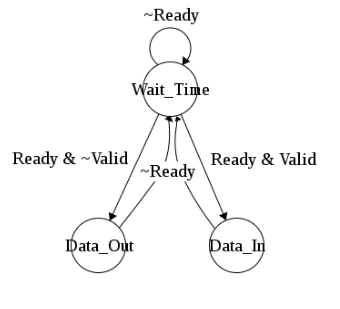
\includegraphics[scale=0.8]{imgs/maquina-estados.png}
    \end{center}
    \legend{Fonte: Produzido pelos autores.}
\end{figure}